\documentclass{article}

\usepackage{tikz}
\usetikzlibrary{shapes.multipart,positioning}

\usepackage{listings}

\begin{document}
  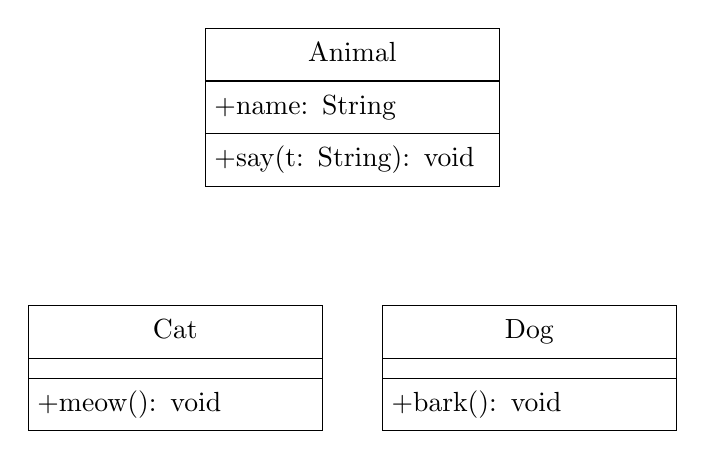
\begin{tikzpicture}[
      shorten >=1pt,
      every text node part/.style={align=center},
      class/.style={
        rectangle split,
        rectangle split parts=3,
        draw,
        text width=3.5cm
      },
      node distance=1.5cm and -1.5cm
    ]
    \node[class]
      (Animal)
      {\strut Animal
      \nodepart{two}
      \strut +name: String
      \nodepart{three}
      \strut +say(t: String): void};
      
    \node[class, below left=of Animal]
      (Cat)
      {\strut Cat
      \nodepart{two}
      \nodepart{three}
      \strut +meow(): void};
      
    \node[class, below right=of Animal]
      (Dog)
      {\strut Dog
      \nodepart{two}
      \nodepart{three}
      \strut +bark(): void};
  \end{tikzpicture}
\end{document}